\chapter{Conclusão}

Nesse capítulo teremos exemplos de figuras, listas, textos em itálico, negrito, notas de rodapé e referências internas ou referência cruzada. 

\section{Exemplos com Figuras}

Texto para iniciar a seção.

Lorem ipsum dolor sit amet, consectetur adipiscing elit. Aliquam eros orci, hendrerit sed pretium sit amet, aliquam sit amet quam. Cras nec dolor ac magna mattis pharetra. Morbi interdum quam nisl, tincidunt egestas nisi tempus at. Quisque pulvinar mi sem, a ultrices nunc scelerisque a. Suspendisse ac risus cursus, pellentesque ex ut, scelerisque tellus. Nullam maximus nisl vel felis dapibus, vel placerat libero congue. Nullam euismod iaculis tincidunt. Vestibulum porta scelerisque vulputate. Vivamus rhoncus, massa ut sodales interdum, velit magna pharetra dui, in fringilla erat sem non metus. 

Conforme exemplo abaixo, é possível incluir imagens lado a lado, como do video game (Figura \ref{fig:videogame}) e da coxinha (Figura \ref{fig:coxinha}).

\begin{figure}[H]
	\centering
	\begin{minipage}[t]{0.45\linewidth}
		\centering
		\caption{Video Game}
		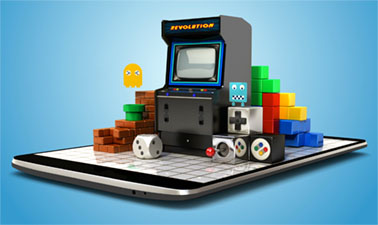
\includegraphics[width=\linewidth]{videoGame.jpg}
		\label{fig:videogame}
		\fonte{\citeonline{VideoGame2017}}
	\end{minipage}
	\hspace{0.2cm}
	\begin{minipage}[t]{0.45\linewidth}
		\centering
		\caption{Coxinha}
		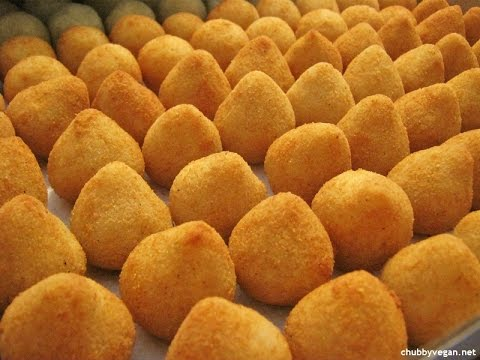
\includegraphics[width=0.8\linewidth]{coxinha.jpg}
		\label{fig:coxinha}
		\fonte{\citeonline{Coxinha2017}}
	\end{minipage}
\end{figure}

Na seção seguinte é apresentado exemplos de listas.


\section{Seção sobre Listas}

A seguir exemplos de 3 tipos de listas. Numerada, com bolinhas e com letrinhas.

\subsection{Lista Numerada}

A seguir exemplos de itens de lista numerada:

\begin{enumerate}[leftmargin=1.7cm]
	\item Sorvete;
	
	\item Coxinha;
	
	\item Pizza;
	
	\item Chocolate.
\end{enumerate}

\subsection{Lista com Bolinhas}

Exemplo de lista com marcadores circulares ou bolinhas:

\begin{itemize}[leftmargin=1.7cm]
	\item Sorvete;
	
	\item Coxinha;
	
	\item Pizza;
	
	\item Chocolate.
\end{itemize}

\subsection{Lista com Letrinhas}

Lista com identificadores com letras do alfabeto:

\begin{enumerate}[label=\alph*), leftmargin=1.7cm]
	
	\item Sorvete;
	
	\item Coxinha;
	
	\item Pizza;
	
	\item Chocolate.
	
\end{enumerate}

Na próxima seção são apresentados exemplos de textos itálicos, negritos e sublinhados.


\section{Textos}

Exemplos de textos \textit{itálicos}, \textbf{negrito} e \underline{sublinhado}:

Pra fazer texto itálico, a gente usa o comando \begin{verbatim} \textit{Palavra em Itálico} \end{verbatim}.

Pra fazer texto negrito, usamos o comando \begin{verbatim} \textbf{Palavra em Negrito} \end{verbatim}.

E para fazer um texto sublinhado, usamos \begin{verbatim} \underline{Palavra Sublinhada} \end{verbatim}.

A próxima seção apresenta exemplos de textos com notas de rodapé.

\section{Nota De Rodapé}

Para fazer uma nota de rodapé, usamos o comando \begin{verbatim} \footnote{Texto que vai no rodapé.} \end{verbatim}.

Aqui um exemplo de nota de rodapé\footnote{Essa é uma nota de rodapé.}.

As notas de rodapé também podem ter citações. O que problema nesse exemplo é que o texto, em um editor LaTeX pode ficar difícil de perceber e alterar\footnote{Essa é uma nota de rodapé que vai no meio do texto e ainda tem uma referência \cite{UTFPR2017}.}, mas ao gerar o PDF, ela fica mais perceptível.

A próxima seção apresenta exemplos de referências cruzadas.

\section{Referenciar Coisas Passadas}

Exemplos de como referenciar seções, imagens e tabelas que estão localizadas antes deste ponto do texto.

Para referenciar algo, é preciso que o que será referenciado tenha um \textit{label} e o local que referencia precisa usar um \textit{ref}.

Exemplo:

Aqui vamos referenciar a imagem do sorvete (Figura \ref{fig:sorvete}) que foi apresentada na seção \ref{sec:outra}.

Aqui vamos referenciar a tabela longa (Tabela \ref{tabela:longa}) que foi apresentada na seção \ref{sec:tabela}.


\section{Referenciar Coisas Futuras}

Também é possível referenciar conteúdos que ainda não foram apresentados, como é o caso desse exemplo que faz referência ao Apêndice (tabela \ref{tabela:tabelinha}), que é uma tabela simples, ou seja, não precisou de mais de uma página para ser apresentada.